
\chapter{Results}

This section details the results of investigations into how point estimates of bathymetry can be extracted from ICESat-2 data, and then how these point estimates can be interpolated and integrated into existing bathymetry grids to produce an upscaled product. Sections \ref{subsec:randomsample} and \ref{subsec:petten_kriging} validate the principle of interpolating point estimates and combining them with GEBCO. In section \ref{subsec:randomsample} random point samples of the validation data for a region are taken, then those points are used as synthetic input data to the kriging + Kalman updating approach. Then, in section \ref{subsec:petten_kriging}, point estimates of bathymetry from JarKus are used as input to the Kriging Kalman updating process. The rest of the chapter shows the results of the full methodology, including ICESat-2 signal finding and the interpolation/updating of the GEBCO data. This full cycle is applied at 4 test sites: Marathon Key (Florida, USA), St.~Croix (US Virgin Islands), St.~Thomas and St.~John (US Virgin Islands), and the Island of Oahu (Hawai'i, USA). Then, the full set of ICESat-2 data points extracted from all test sites are aggregated to evaluate if there are any variables which predict the quality or availability of bathymetric signal in the ICESat-2 data.

The global distribution of the test sites where the full cycle is implemented is shown in Figure \ref{fig:world-site-map}

\begin{figure}[!ht]
    \centering
    \includegraphics[width=0.8\textwidth]{figures/all_site_overview_map.pdf}
    \caption{All test sites where the full methodology was implemented and validated}
    \label{fig:world-site-map}
\end{figure}

\section{Kriging and Kalman update validation by random sampling}\label{subsec:randomsample}

The basic approach behind both the kriging interpolation method and Bayesian updating of GEBCO is validated using a synthetic experiment. Instead of using point data from ICESat-2 as an input to the kriging step, random point samples of the validation data are taken throughout a single area of interest. This provides a source of exact bathymetry point measurements with an RMSE of 0 m. Two types of random sampling are considered, randomly across the surface of the validation data, and colinear samples that are taken only along the corresponding ICESat-2 tracks. The latter simulates the availability of theoretical perfect measurements from ICESat-2 bathymetry data, and can be compared to the random sampling case to investigate the effect of sparse, irregular spacing of data points induced by the satellite tracklines. Any available ICESat-2 bathymetric data will occur along colinear track lines, and therefore there will always be some spatial gaps in the data even if perfect ICESat-2 data were present along every single tract. By comparing the randomly sampled points to colinear points sampled along the ICESat tracks, we can get an estimate of how much the accuracy is degraded by the data being available only along certain lines.

A small section of the St.~Croix validation data is used to implement this trial. First, the raster of the validation data is sampled randomly until we have a set of $10^4$ random data points. From this set a subsample of $2000$ points is taken using the Poisson disk sampling method. This subsample is used as input to the kriging algorithm.

Figure \ref{fig:truthras-sampling} shows both sets of points that were used as input to the kriging process for the two cases under evaluation. Note that in the bottom figure there are significant spatial gaps in coverage. This is due to the pattern of ICESat-2 data collection. Even in this theoretical scenario with exact bathymetry values available across the entire track, the spatial anisotropy of the availability of the points can potentially limit the accuracy of the interpolation.

\begin{figure}[h]
    \centering
    \includegraphics{figures/truthraster_sampling_combined.pdf}
    \caption[Random sampling points for validation test]{Top: Random sampling across the area of interest \newline  Bottom: Random sampling only along the ICESat-2 tracks for the site}
    \label{fig:truthras-sampling}
\end{figure}

Because we know the bathymetry points used for this section are exactly the same as the validation data at each point, the \emph{nugget} of the variogram for the Kriging interpolation is set to $0$, so areas that are close known points are given a variance of $0$ by the kriging process.
\begin{table}
\caption{Error between the various data products}
\label{tab:rmse-truth-raster-sampled}
\begin{tabular}{lrr}
 & RMSE & MAE \\
Truth vs 50m bilinear resampling of GEBCO & 6.200386 & 4.697360 \\
Truth vs Kriged raster output & 2.435478 & 1.275817 \\
Truth vs GEBCO+Kriged raster & 1.682143 & 1.057158 \\
\end{tabular}
\end{table}


Table \ref{tab:random-vs-colinear-sampling} shows the results of the two sampling strategies. It can be seen that the more homogenous distribution of bathymetric points in the randomly-sampled data produces a better kriging estimate (RMSE of 3.13~m and 4.49~m respectively).

Also of note is that for both cases, the Bayesian combination of the kriging surface with GEBCO produces a better estimate than either on their own. This indicates that there is value in starting from GEBCO and using a Bayesian combination approach when compared to either a kriging interpolation of point data or using GEBCO as a data source.


\section{Petten Test Site}\label{subsec:petten_kriging}
Most research results show that spaceborne lidar is not effective at retrieving bathymetry from very turbid waters \parencite{Daly2022,Coveney2021a}. To test the upper limits of this, ICESat-2 data for the coast of Petten, NL was downloaded. As expected, there was no bathymetric signal found in the ICESat-2 data, likely due to the inability of the laser to penetrate the turbid water.

However the site provides a useful case to validate the approach of the combination of universal kriging of point bathymetry and Bayesian combination of bathymetry grids. The Dutch government provides a dataset called JarKus which consists of annual surveyed elevations of the coastal zone \parencite{Minneboo1995}. These point measurements provide an interesting case to apply the same method but using the Jarkus point measurements as an input instead of ICESat-2 point measurements.

The location of Petten, The Netherlands, located on the Noord-Holland coast, was chosen based on the availability of high-resolution ground-truth bathymetry provided by Van Oord. The survey was performed in 2021, and therefore the 2021 Jarkus points were selected from the dataset. All Jarkus points that overlap the validation data raster were selected. Like the ICESat-2 data points, the Jarkus points are available only along colinear lines. This is due to the measurement method that is based on surveying the dune and seabed starting from a series of fixed measurement poles and then surveying points normal to the shore starting at the reference pole.

% \begin{figure}
%     \begin{floatrow}
%         \ffigbox{ 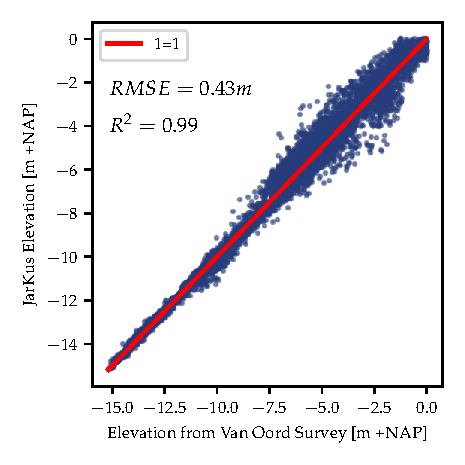
\includegraphics{figures/petten_lidar_estimated_vs_truth.pdf}}{  \caption{Petten Test site: Agreement between Jarkus and Van Oord multibeam survey data}    \label{fig:petten-bias-plot}}
%         \ffigbox{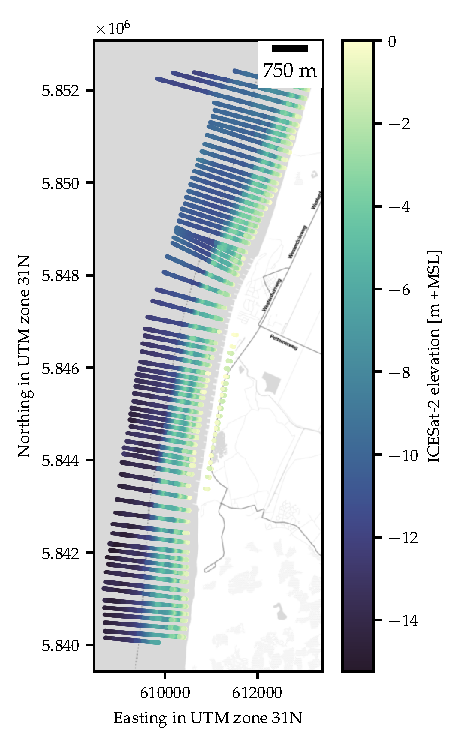
\includegraphics[]{figures/Petten_photon_map.pdf}}{ \caption{Jarkus 2021 measurement points within the site}\label{fig:jarkus-points}}
%     \end{floatrow}
% \end{figure}

\begin{figure}[ht]
    \centering
    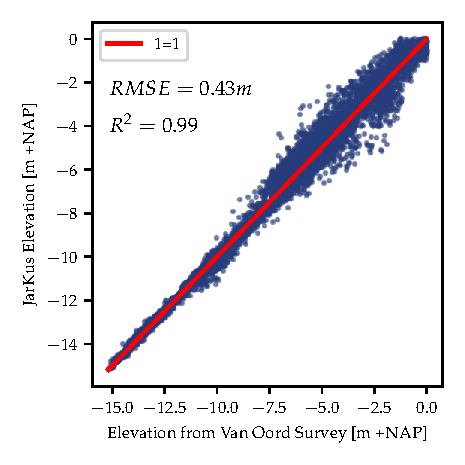
\includegraphics{figures/petten_lidar_estimated_vs_truth.pdf}
    \caption{Petten Test site: Agreement between Jarkus and Van Oord multibeam survey data}    \label{fig:petten-bias-plot}
\end{figure}

\begin{figure}[ht]
    \centering
    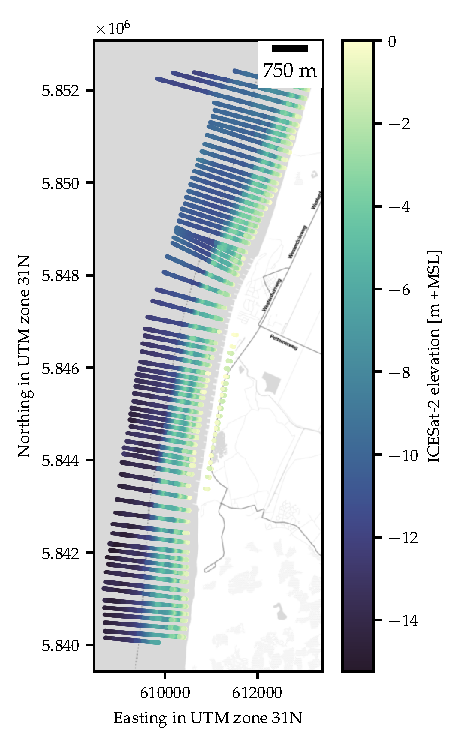
\includegraphics[angle=-90]{figures/Petten_photon_map.pdf}
    \caption{Jarkus 2021 measurement points within the site}\label{fig:jarkus-points}
\end{figure}


The Jarkus point measurements were checked for the same error metrics as the ICESat-2 points. The bias plot is shown in Figure \ref{fig:petten-bias-plot}. It is notable that the deviation between the Jarkus data and the survey data is greatest in the in the shallowest part of the nearshore zone; this is likely due to some morphological changes due to wave-driven sediment exchange between the nearshore and the offshore. Both datasets are from 2021, but this area is highly morphologically active. Also, in the deeper part of the study area, the error between the two datasets decreases significantly. This is likely due to the depth of closure for most profiles in the study area being located between -5 and -10 m.

The Jarkus points are used as input to the kriging process instead of ICESat-2 points to validate the universal kriging and Kalman updating process at this site. 

\begin{figure}[!ht]
    \begin{floatrow}
        \ffigbox{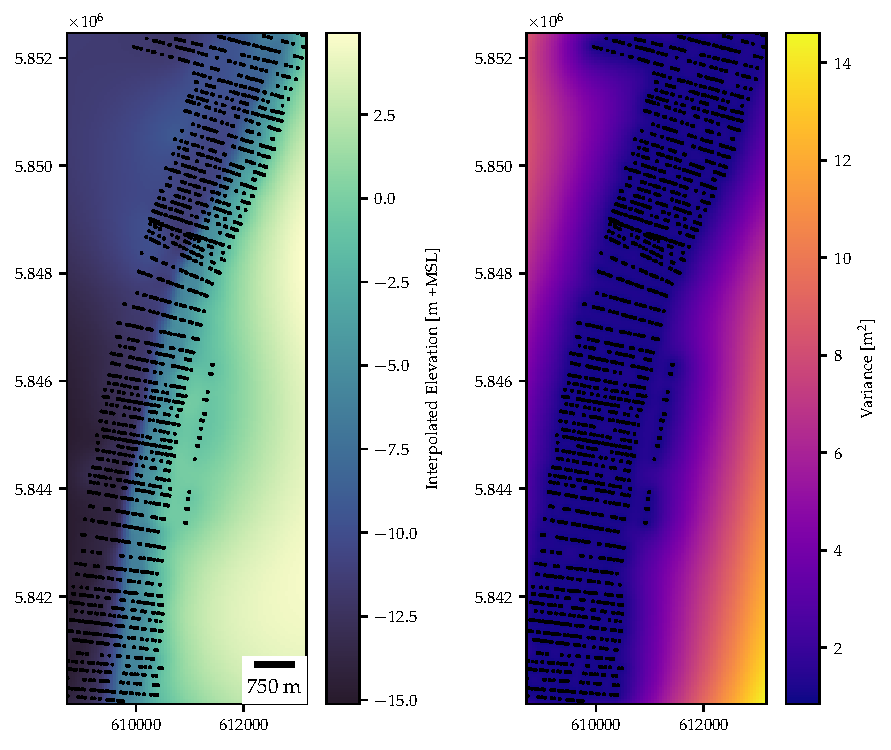
\includegraphics[width=0.5\textwidth]{figures/Petten_kriging_output.pdf}}{\caption{Petten site: result of kriging interpolation}\label{fig:petten-kriging}}
        \ffigbox{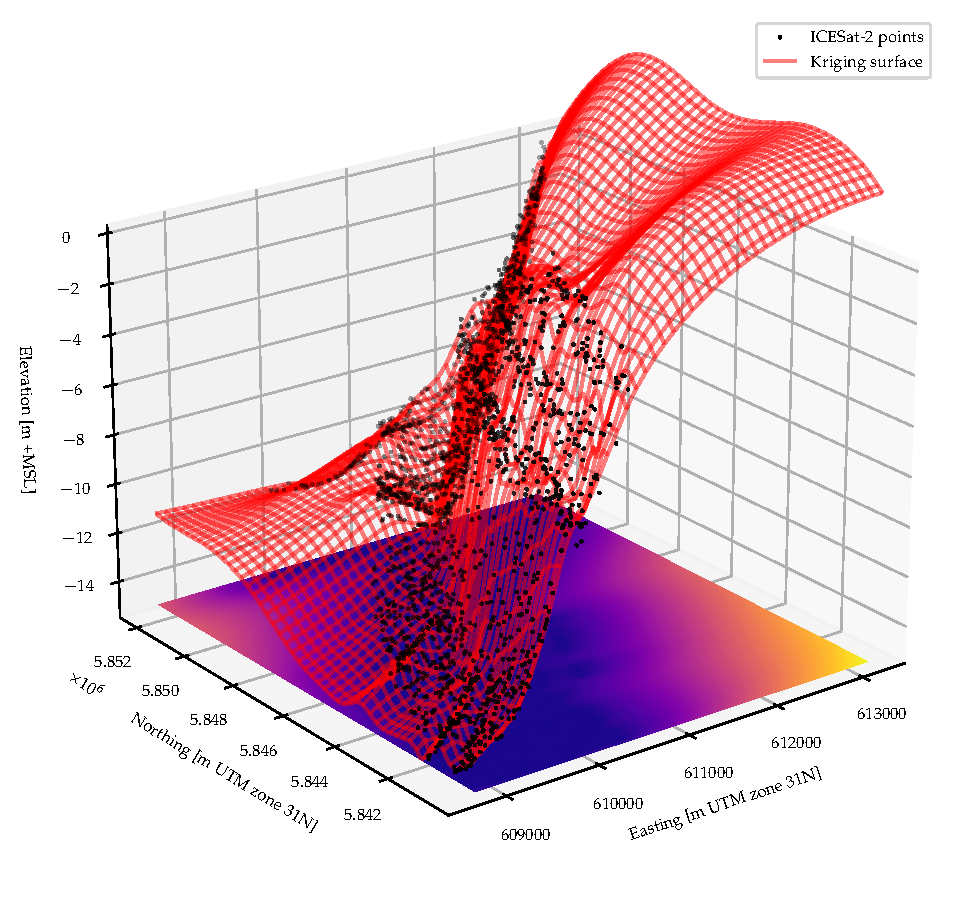
\includegraphics[width=0.5\textwidth]{figures/Petten_plot_3d.pdf}}{\caption{3D results at Petten site}\label{fig:petten-3d-plot}}
    \end{floatrow}    
\end{figure}

The kriging output is shown in Figures \ref{fig:petten-kriging} and \ref{fig:petten-3d-plot}. The Jarkus points show an even distribution of measurement points in the cross-shore and alongshore directions in the entire study site, so the RMSE between the kriging output surface is very low. This site is also very well-suited to interpolation, since the bathymetry of the site is relatively homogenous and isotropic - the slopes and elevations are all relatively constant. Because this nearshore area has good quality point data and also is easy to interpolate, the kriged bathymetry surface was found to have a lower RMSE and MAE error than GEBCO. 

It is notable that in this site, the error between GEBCO and the high resolution bathymetry is significantly lower than other test sites. This could be due to higher quality or more recent input data into the GEBCO grid as compared to the other sites. Even with a higher accuracy in the GEBCO data it was found that the Bayesian combination of both of these datasets has the highest accuracy --- indicating that the Bayesian combination of these two datasets increases the value compared to either dataset individually.

\begin{table}[!ht]
\centering
\caption{Improvement in error metrics after applying Kalman Updating of kriged data}
\label{tab:Petten_gebco_raster_error}
\begin{tabular}{lrrr}
\toprule
 & RMSE [m] & MAE [m] & ME [m] \\
\midrule
GEBCO & 1.48 & 1.31 & -1.01 \\
Kriging Surface & 1.22 & 0.70 & -0.31 \\
Kalman Output& 1.00 & 0.76 & -0.50 \\
\bottomrule
\end{tabular}
\end{table}



\section{Florida Keys test site}

% \pdfcomment{talk about the validation data for the site}

The area surrounding Marathon Key in the Florida Keys archipelago in Florida, USA was used as one site to test the entire process, including the ICESat-2 signal finding in additional to the kriging and Kalman updating. The area has a wide and relatively shallow ($\sim -10 m +MSL$) shelf, a microtidal tidal environment, and very clear water, so it is an ideal site for remote sensing of bathymetry. The clear and shallow water provides a relatively strong subsurface signal within ICESat-2 transects. The site was found to have many transects of ICESat-2 data with distinct bathymetric signal. The KDE signal finding approach was applied to all transects within the study area and resulting distribution of the identified signal points is shown in Figure \ref{fig:keys-photons}.

\begin{figure}[!ht]
    \centering
    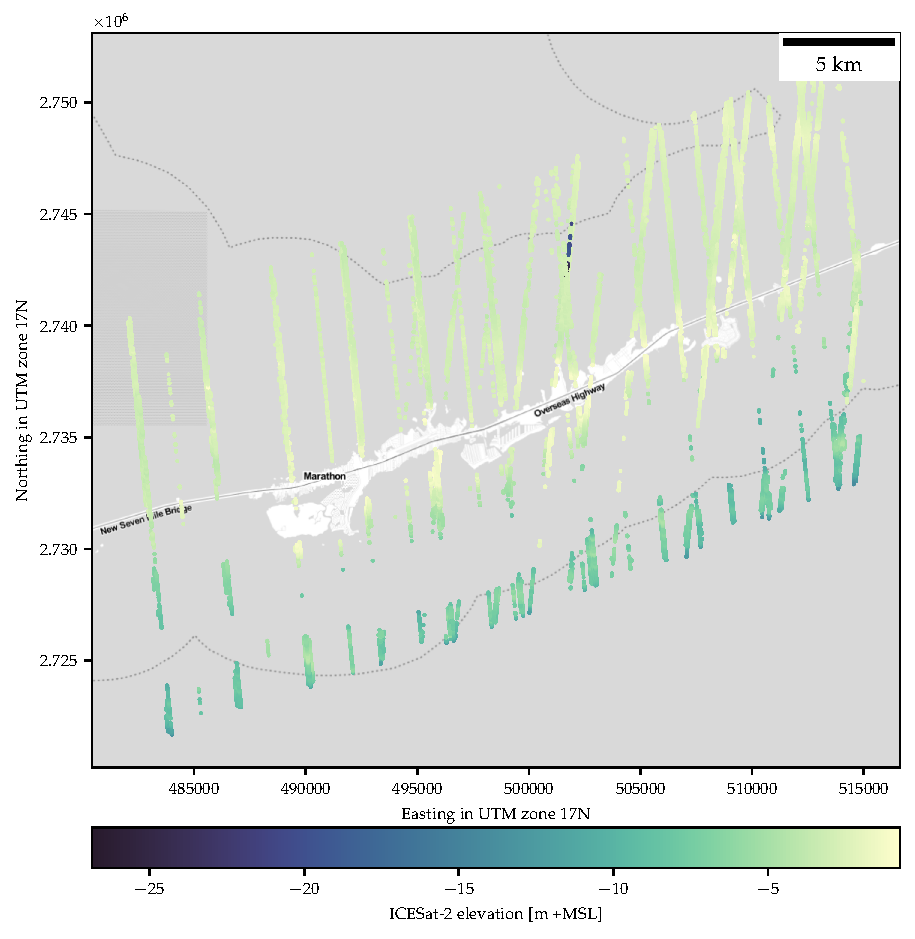
\includegraphics[width=0.8\textwidth]{figures/florida_keys_photon_map.pdf}
    \caption{Marathon Key Site: Location and depth of bathymetric signal points found using KDE signal finding method}
    \label{fig:keys-photons}
\end{figure}

\begin{figure}[!ht]
    \centering
    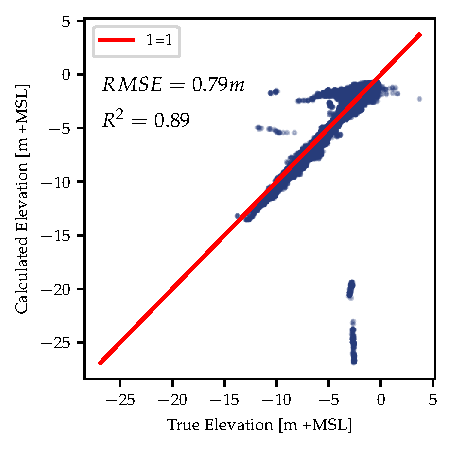
\includegraphics{figures/florida_keys_lidar_estimated_vs_truth.pdf}
    \caption[Marathon Key site: Error bias plot]{Marathon Key site: Bias plot showing the results of the KDE signal finding algorithm}
    \label{fig:keys-biasplot}
\end{figure}

Figure \ref{fig:keys-biasplot} shows how the error is distributed within the Florida Keys test site. This site has many transects containing data, but some errors in the signal finding can be seen in this bias plot. There is one cluster of points with a real elevation of -2.5 m, while the KDE finding output identifies the seafloor elevation as between -20 and -27 m. This is caused by data being missing along this transect in one area. For this location, all photons above -15 m MSL are completely missing from the data. This is likely due to data quality issues, such as the onboard computer not being able to correctly identify the elevation of the primary surface return and opening another telemetry band. The figure also shows a few clusters of points where the seabed location was overestimated slightly. These errors are due to some places where the filtering step did not fully remove the ocean surface signal, which can bias the KDE signal finding algorithm by adding strong signal near the surface, which causes the algorithm to find the density peak higher in the water column than it should appear.

However, the kriging process can account for an expected degree of error, and can be set up such that the input points are not considered exact measurements but are considered to have their own uncertainty at each point. This is controlled by the \emph{nugget} variogram parameter.

\begin{figure}[!ht]
\begin{floatrow}
        \ffigbox{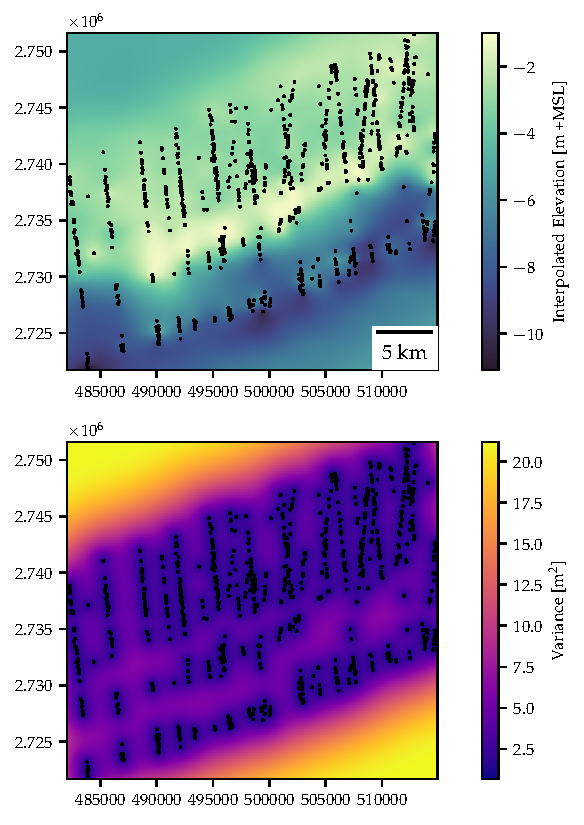
\includegraphics[width=0.5\textwidth]{figures/florida_keys_kriging_output.pdf}}{\caption{Output of the kriging process for the marathon key test site}\label{fig:marathon-key-kriging}}
        \ffigbox{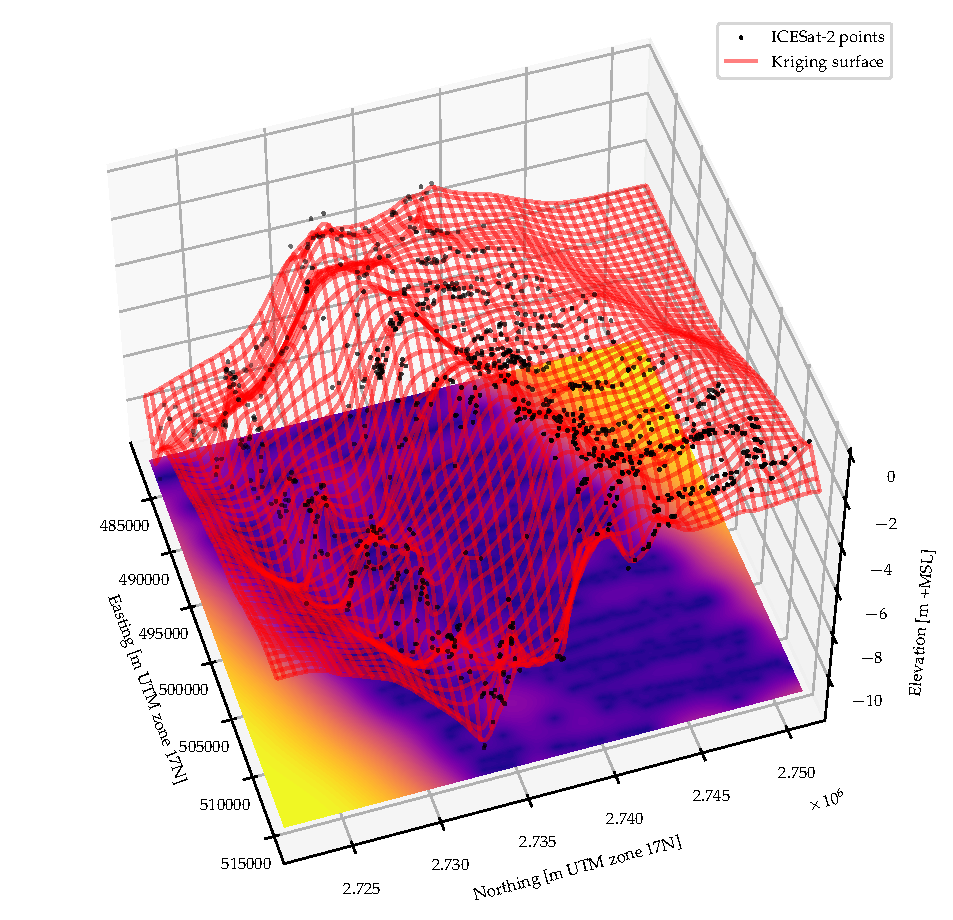
\includegraphics[width=0.5\textwidth]{figures/florida_keys_plot_3d.pdf}}{\caption{The Results of the kriging process in 3D}\label{fig:florida-3d}}
\end{floatrow}
\end{figure}


The Kriging interpolation results are shown in Figures \ref{fig:florida-3d} and \ref{fig:marathon-key-kriging}.

The change in error after the Kalman updating step is shown in table \ref{tab:florida_keys_gebco_raster_error}, and the spatial distribution of this improvement is shown in Figure \ref{fig:fl-keys-improvement}. At this site the largest improvements actually happen on the edges of the available spaceborne lidar data. The kriging surface that has been fit through these points happens to match the validation data well along these points. Also, notably this improvement occurs along a change in the GEBCO source data for this site.

\begin{figure}[!ht]
    \begin{floatrow}
        \ffigbox{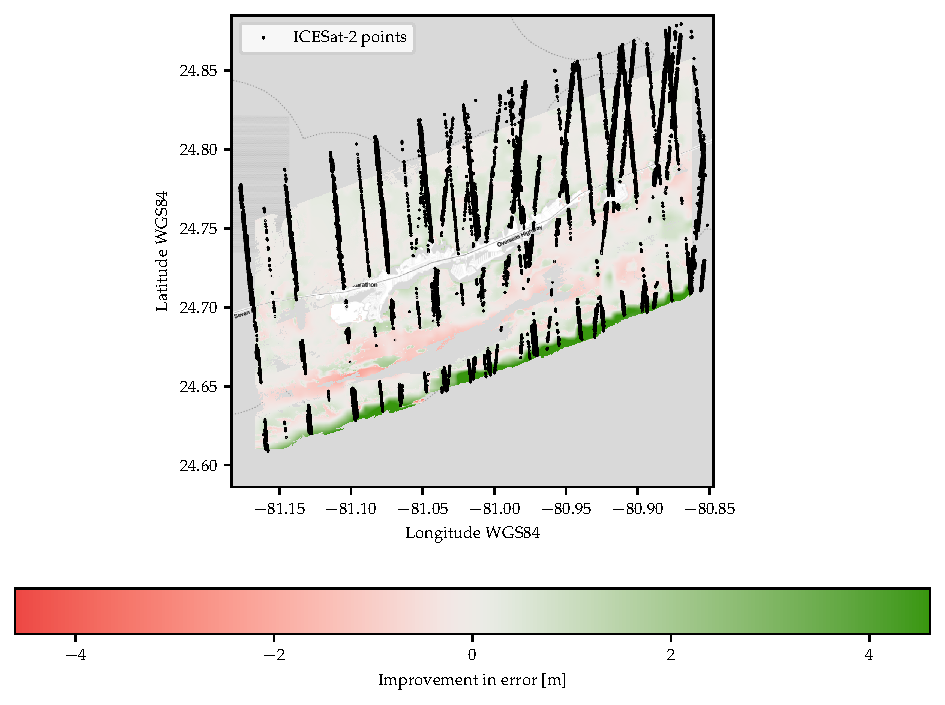
\includegraphics[width=0.5\textwidth]{figures/florida_keys_error_improvement.pdf}}{\caption{Improvement in error after application of Kalman updating}\label{fig:fl-keys-improvement}}
        \capbtabbox{\input{tables/florida_keys_kalman_improvement.tex}}{\caption{Improvement in error metrics after applying Kalman updating of kriged data}\label{tab:florida_keys_gebco_raster_error}}
    \end{floatrow}
\end{figure}

\section{St.~Croix test site} \label{sec:stcroix-site}

Another site where the entire processing chain was implemented was in the Caribbean island of St. Croix. The site was chosen based on the availability of recent high-resolution bathymetry validation data, and also on the basis of the clear water. The site provides some interesting contrasts: the south edge of the island is a relatively gently sloping shelf, while the north edge of the island has an extremely steep shoreline. On the northeast edge there is a bank between the main island and a smaller island.

The validation data used is provided by a USGS-sponsored survey of the area using a Riegl VQ-880-G II lidar sensor between January and June 2019. The lidar point data was then post-processed into a 1 m raster DEM product with a bathymetric vertical accuracy of $12.1$~cm when compared to the survey control points \parencite{USVI-lidar2022}. This DEM was used for validation. Note that the areas to the Northwest of the island has a very steep slope, and is therefore missing in the validation data - the slope is steep enough that the airborne lidar sensor could not get sufficient signal in that area.

\begin{figure}[!ht]
    \centering
    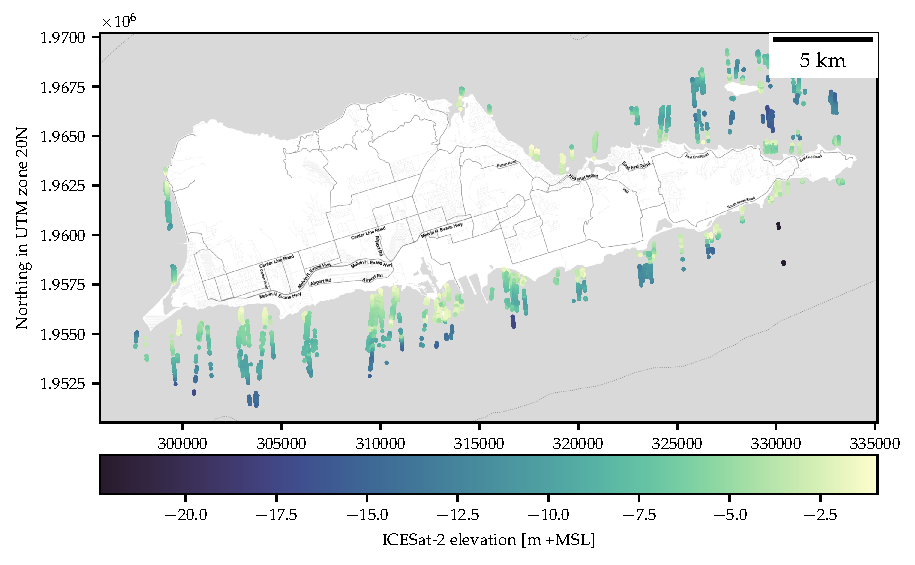
\includegraphics{figures/stcroix_photon_map.pdf}
    \caption{St.~Croix site: Identified photons and their depth}
    \label{fig:st-croix-photons}
\end{figure}

The bathymetric point measurements obtained from the KDE signal finding algorithm are shown in \ref{fig:st-croix-photons}. This site showed excellent agreement between the ICESat-2 data and the validation data, and the KDE signal finding algorithm reliably identified bathymetric points as deep as -20~m +MSL. The overall RMSE at the site was the lowest of any sites tested, at 0.54 m. Figure \ref{fig:st-croix-bias-plot} shows the spread of the ICESat-2 points vs the corresponding point in the validation data. Just as in the validation data, the north west slope of the island does not contain any signal.

\begin{figure}[!ht]
    \centering
    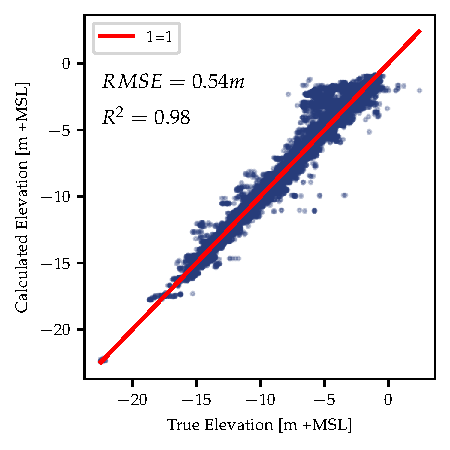
\includegraphics{figures/stcroix_lidar_estimated_vs_truth.pdf}
    \caption{St.~Croix site: Error Bias plot}
    \label{fig:st-croix-bias-plot}
\end{figure}

The results of the kriging output for this site are shown in Figures \ref{fig:stcroix-kriging} and \ref{fig:stcroix-3d}. Because the north end of this site has a very steep slope, there is no bathymetric signal found in this area and the resulting uncertainty is very high in this region. The south end of the island has a more gentle slope and there is a significant amount of bathymetric data available, so it has a correspondingly higher confidence in the kriging estimate.

\begin{figure}[!ht]
    \begin{floatrow}
        \ffigbox{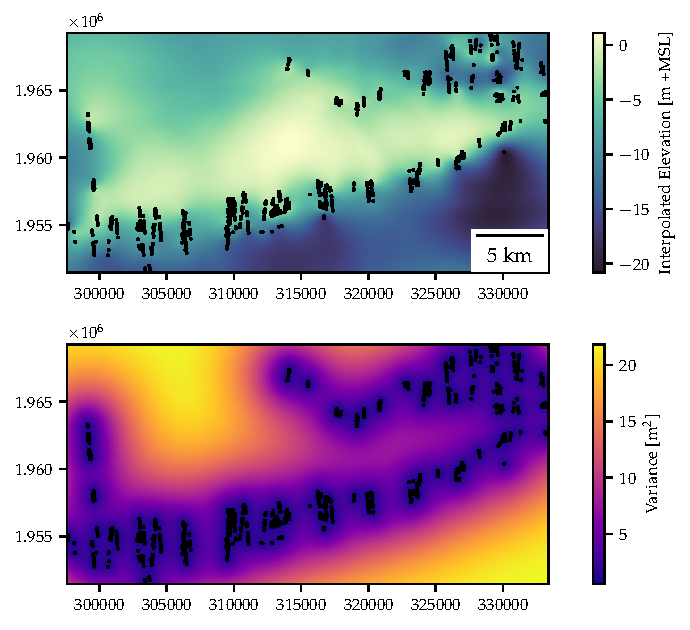
\includegraphics[width=0.45\textwidth]{figures/stcroix_kriging_output.pdf}}{\caption{Results of Universal Kriging interpolation in the St. Croix Test site}\label{fig:stcroix-kriging}}
        \ffigbox{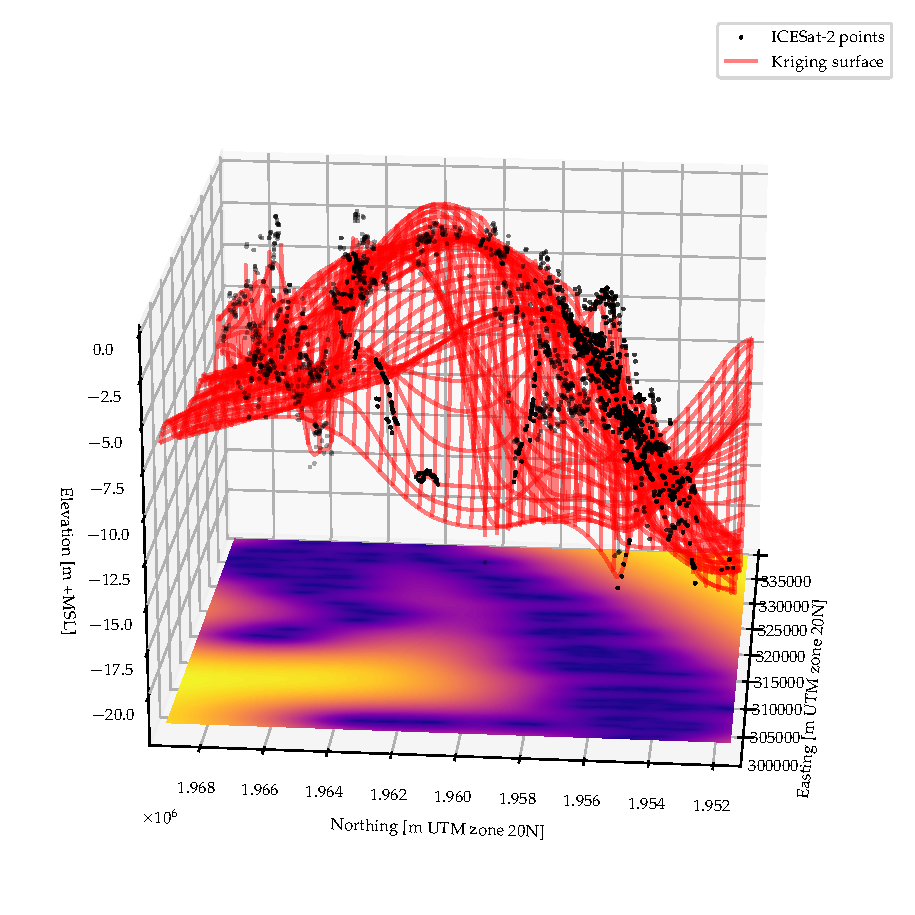
\includegraphics[width=0.45\textwidth]{figures/stcroix_plot_3d.pdf}}{\caption[3D Plot of the kriging result at St. Croix Site]{3D Plot of the kriging results (red wireframe) with the resulting uncertainty shown on the bottom of the plot. Note that the scale of the uncertainty (plotted on the bottom) is the same used in the lower half of \ref{fig:stcroix-kriging}}\label{fig:stcroix-3d}}
    \end{floatrow}
\end{figure}

After implementing the Kriging/Kalman updating process for the St.~Croix site it is found that the combination of the kriged ICESat-2 raster with the GEBCO data produces a resulting product that has a higher accuracy than either of the input datasets. Particularly notable here is the inaccuracy of the GEBCO data at this site --- while the overall RMSE of the resulting raster is high at this site compared to some others, in this case it is limited by the accuracy of the starting GEBCO data, and the accuracy of the kriging raster. Table \ref{tab:stcroix_gebco_raster_error} shows the error metrics for the site for the three bathymetric grids, and the spatial distribution of the improvement in error is shown in Figure \ref{fig:improvement-st-croix}. The improvement in error is also well-distributed within areas that contain bathymetric signal, with the largest improvements in error having a magnitude of about 6 meters. In some areas, there was a minor increase in absolute error. These areas are mostly in places where the bathymetric points are not evenly spatially distributed.


\begin{figure}[htbp]
    \begin{floatrow}
        \ffigbox{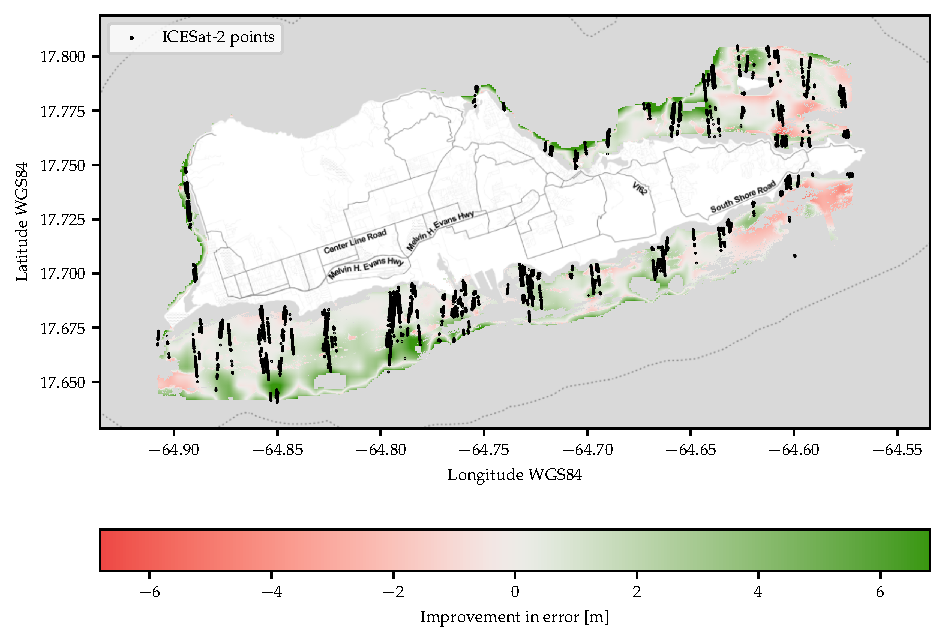
\includegraphics[width=0.5\textwidth]{figures/stcroix_error_improvement.pdf}}{\caption[Spatial distribution in error improvement at St. Croix site]{Improvement in absolute error in meters after combining the interpolated bathymetry grid via Kalman updating. The improvement at this site occurs mostly at the middle depths. A larger version of this figure is shown in \ref{fig:site-stcroix-error-improvement-appendix}}\label{fig:improvement-st-croix}}
        \capbtabbox{\begin{table}
\centering
\caption{Improvement in error metrics after applying Kalman Updating of kriged data}
\label{tab:stcroix_gebco_raster_error}
\begin{tabular}{lrrr}
\toprule
 & RMSE [m] & MAE [m] & Mean Error [m] \\
\midrule
Naive Bilinear Interpolation & 6.45 & 4.30 & -1.01 \\
Kriged Raster & 6.79 & 4.10 & -2.91 \\
Kalman Updated Raster & 4.63 & 3.20 & -1.14 \\
\bottomrule
\end{tabular}
\end{table}
}{\caption{Improvement in error metrics after applying Kalman updating of kriged data}\label{tab:stcroix_gebco_raster_error}}
    \end{floatrow}
\end{figure}



\section{St.~Thomas and St.~John test site}
Another test site used to evaluate the ICESat-2 bathymetry signal finding steps is area around the islands of St.~Thomas and St.~John, located in the U.S.~Virgin Islands. The islands are ideal for spaceborne bathymetry for the same reason that many Caribbean islands are: they have naturally clear water that is easily penetrated by lidar signal. Additionally, the area has recent, high-resolution bathymetric data available from NOAA to allow validation of the approach. The validation data for the site is from the same surveying project described in Section \ref{sec:stcroix-site}. Because the bathymetric DEM is continuous between the two islands, the two islands were considered as a single test site.

The ICESat-2 data was downloaded for an area of interest that includes extent of the validation data around both islands. Figure \ref{fig:charlotte-amalie-photons} shows the signal that was identified from the ICESat-2 transects at the site. Figure \ref{fig:charlotte-amalie-biasplot} shows the error between the ICESat-2 points and the validation data. There is a cluster of several points on the right side of the plot that shows points with a true elevation of between 10--20~m. This is due to several land points being incorrectly identified as bathymetric signal, which significantly increases the RMS error at the site.

The lidar bathymetric points in this site are moderately well distributed, but each identified cluster of signal is smaller. This is due to the very steep slope of the underlying bathymetry. This steep slope also affects the quality of the bathymetric data around the site. The offshore extent of the bathymetric data is relatively small, because in most directions the depth increases to beyond the maximum depth of the airborne lidar very quickly.

\begin{figure}[!htb]
    \centering
    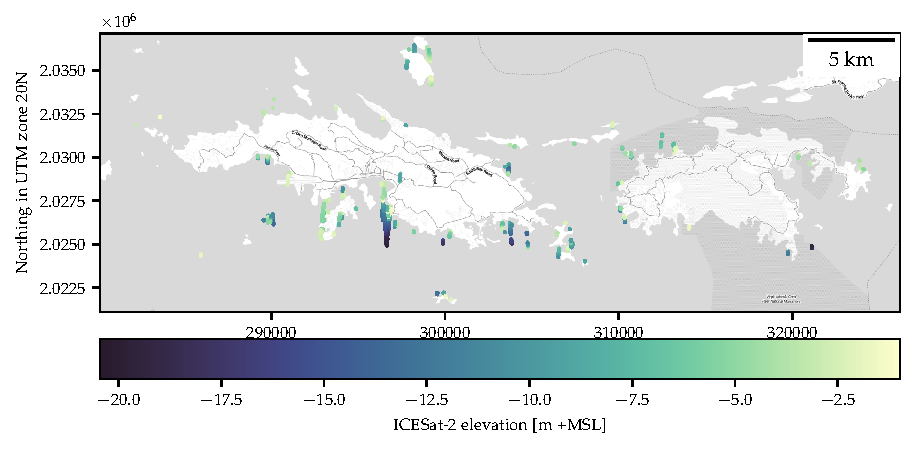
\includegraphics{figures/charlotteamalie_photon_map.pdf}
    \caption{St.~Thomas and St.~John test site: Location and depth of bathymetric signal points found using KDE signal finding method}
    \label{fig:charlotte-amalie-photons}
\end{figure}

\begin{figure}[htbp]
    \centering
    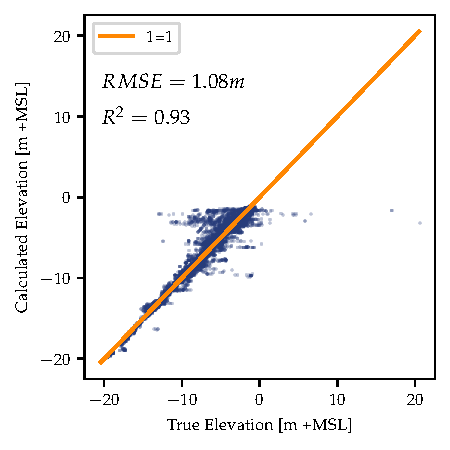
\includegraphics{figures/charlotteamalie_lidar_estimated_vs_truth.pdf}
    \caption{St.~Thomas and St.~John Test site: Bias plot showing the error of ICESat-2 bathymetric signal}
    \label{fig:charlotte-amalie-biasplot}
\end{figure}

The bathymetric points found via the KDE signal finding process were then interpolated using universal kriging interpolation. The interpolated surface is shown in the upper half of Figure \ref{fig:charlotte-amalie-kriging-out} and in the wireframe surface shown in Figure \ref{fig:charlotte-amalie-3d}. This site shows many high-accuracy point estimates in deeper areas of the site (as can be seen in Fig. \ref{fig:charlotte-amalie-biasplot}). However, these points are relatively isolated so confidence in the kriged bathymetry estimate falls off quickly. Also since the clusters of signal have large gaps between them, the accuracy of the fitted curves is likely reduced since trends cannot be estimated as accurately as they would be if there was more intermediate points between the clusters.

\begin{figure}[!ht]
    \begin{floatrow}
        \ffigbox{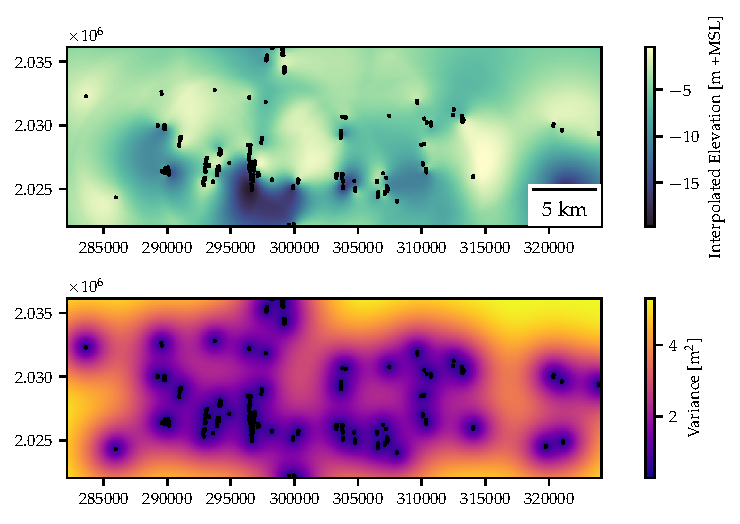
\includegraphics[width=0.45\textwidth]{figures/charlotteamalie_kriging_output.pdf}}{\caption{
            St.~Thomas and St.~John Test site: result of Kriging interpolation
            }\label{fig:charlotte-amalie-kriging-out}}
        \ffigbox{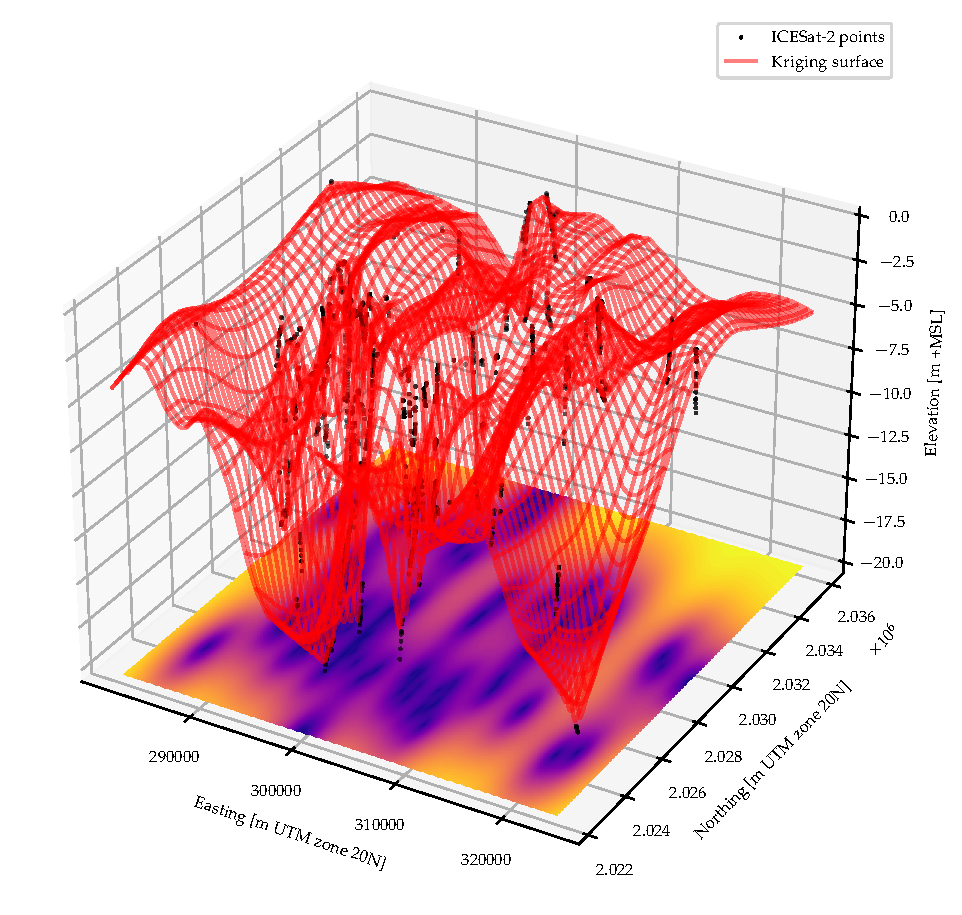
\includegraphics[width=0.45\textwidth]{figures/charlotteamalie_plot_3d.pdf}}{\caption{St.~Thomas and St.~John Test site: 3D results of the kriging interpolation}\label{fig:charlotte-amalie-3d}}
    \end{floatrow}
\end{figure}

After the Kalman updating of the GEBCO bathymetry data, the RMS error was reduced from 7.35 m to 5.78 m. The spatial distribution of the improvement is shown in Figure \ref{fig:charlotte-amalie-improvement}. In some areas, the absolute error is improved by up to 7.5 m compared to the GEBCO data. 
\begin{figure}[!ht]
    \begin{floatrow}
        \ffigbox{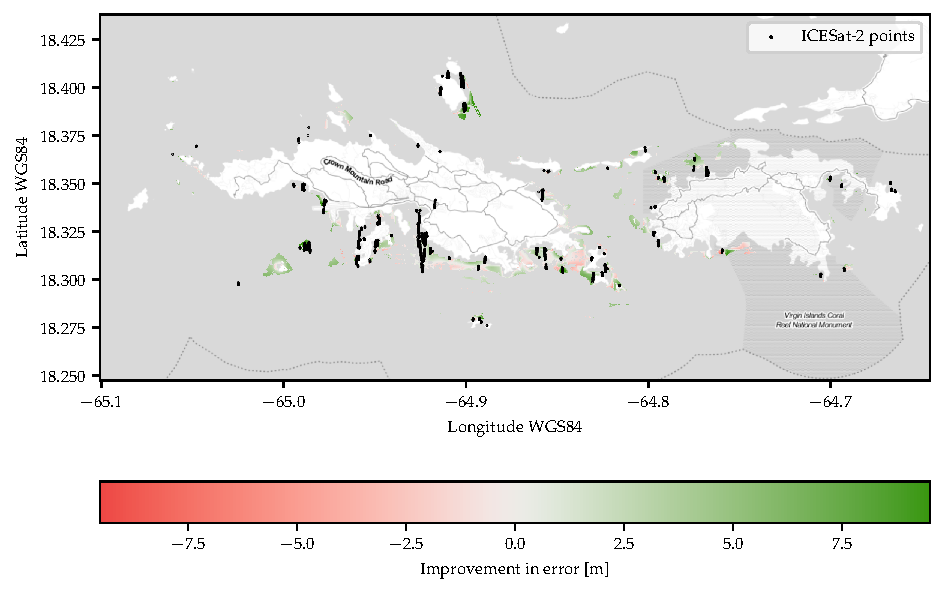
\includegraphics[width=0.45\textwidth]{figures/charlotteamalie_error_improvement.pdf}}{\caption[Absolute error improvement at St.\ Thomas and St.\ John test site]{St.~Thomas and St.~John Test site: Improvement in absolute error [m] after Kalman update. Note the relatively limited offshore extent of the validation data}\label{fig:charlotte-amalie-improvement}}
        \capbtabbox{\input{tables/charlotteamalie_kalman_improvement.tex}}{\caption{Improvement in error metrics after applying Kalman updating of kriged data}\label{tab:charlotteamalie_gebco_raster_error}}
    \end{floatrow}
\end{figure}

\section{Oahu Test sites}\label{sec:oahuresults}

For another validation site that is outside of the Caribbean sea, the island of Oahu in the US state of Hawai'i was chosen. The validation data used is a lidar survey completed in 2013. The nearshore zone was surveyed by the United States Army Corps of Engineers (USACE) using the Coastal Zone Mapping and Imaging Lidar (CZMIL). The survey data was collected by aircraft from September to November 2013. The raw lidar point cloud data was then further processed into a 1 m DEM via TIN interpolation. The resulting 1 m DEM is referenced to a horizontal datum of NAD83(PA11), and the vertical reference system is the local mean sea level. The data has a vertical accuracy at the 95\% confidence interval of $\sqrt{0.20^2 + (0.013d)^2}$~m, where $d$ is the depth in meters. This translates to a 95\% confidence vertical accuracy of $\pm 28$ cm at a depth of 15~m.

Because the island of Oahu is substantially larger than the other test sites ($\approx 4x$ the area), the coast of the island is first divided into 8 smaller subsites to allow for easier data downloading and processing. The layout of these sites was chosen based on approximately similar coastline characteristics, and to try to minimize any interpolation over convex points in the coast. Only some selected sites are highlighted here. Other sections  Figure \ref{fig:oahu-subsite-layout} shows the selected layout of the subsites along the coast of Oahu.

\begin{figure}[htbp]
    \centering
    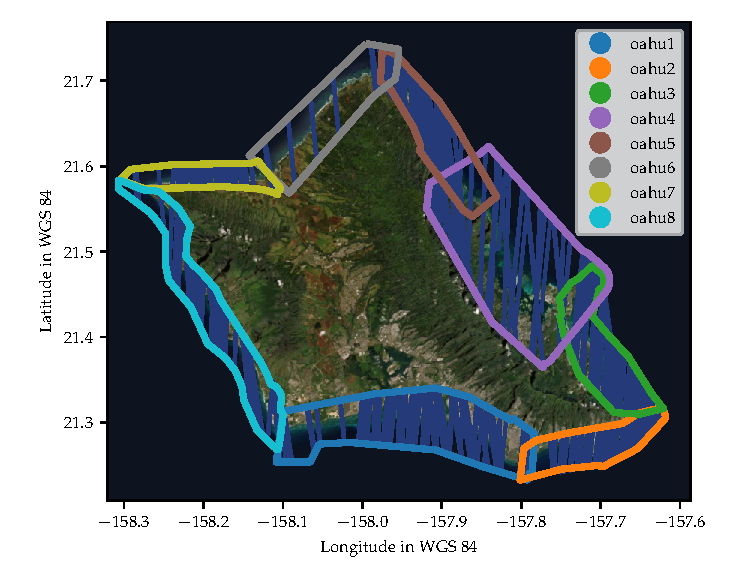
\includegraphics{figures/Oahu_all_tracklines.pdf}
    \caption[Oahu test site: Transects and subsite layout]{Oahu test site: The availability of ICESat-2 transects within the selected subsites. Base layer data provided by: Esri, i-cubed, USDA, USGS, AEX, GeoEye, Getmapping, Aerogrid, IGN, IGP, UPR-EGP, and the GIS User Community}
    \label{fig:oahu-subsite-layout}
\end{figure}

The different subsites also exhibit different hydraulic characteristics. The Northern edge of the island is exposed to longer swells and larger wave heights, while the south is relatively sheltered \parencite{Vitousek2008a}. Another aspect is that distribution of ICESat-2 tracks is not even across all sites. As seen in Figure \ref{fig:oahu-subsite-layout}, sites 4 and 6 do not contain any transects going in the other direction with good data, so distribution of the data will be more uneven and might reduce the quality of the kriging raster.

The accuracy of the ICESat-2 bathymetry points from the KDE signal finding algorithm, grouped by subsite, are shown in Table \ref{tab:Oahusitestats}. It can be seen that site 2 has an anomalously high RMS error.

\begin{figure}[htbp]
    \centering
    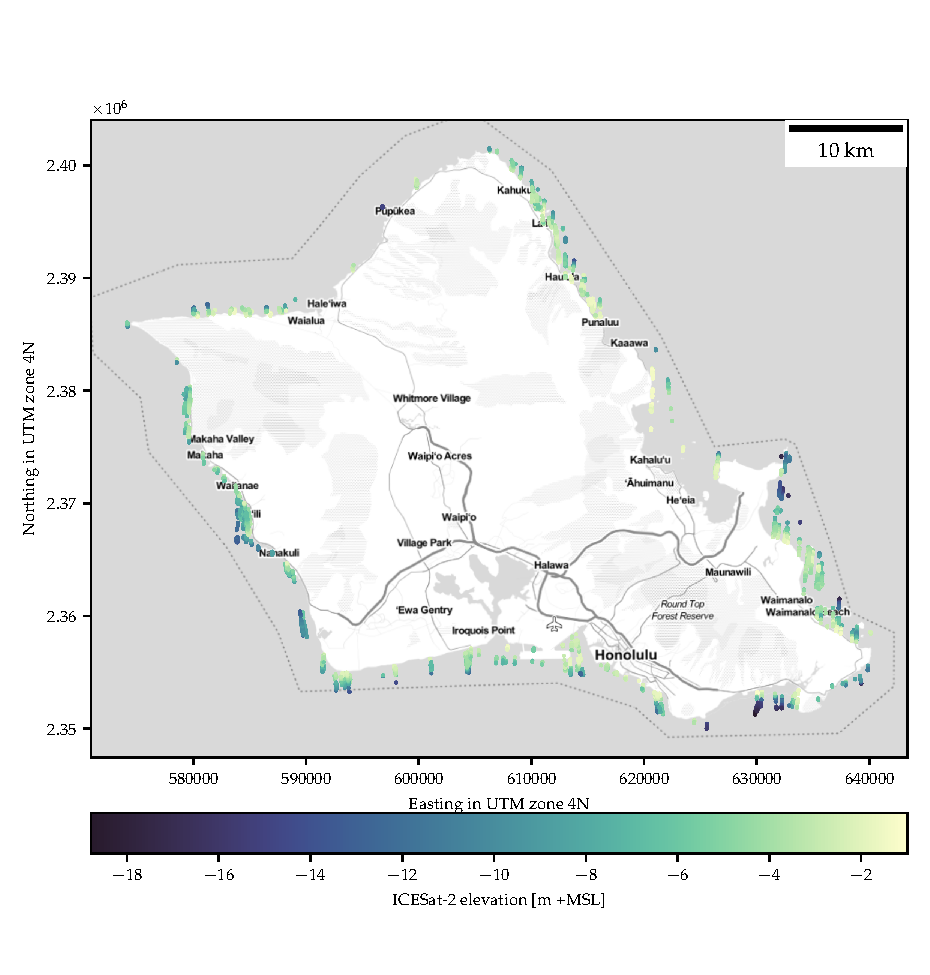
\includegraphics{figures/Oahu_all_sites_photon_points.pdf}
    \caption{Bathymetry point estimates around Oahu from KDE signal finding algorithm}
    \label{fig:oahu-photon-map}
\end{figure}


\begin{figure}
    \begin{floatrow}
        \capbtabbox{% \begin{table}[htbp]
% \centering
% \caption{Percent reduction in error metrics via the Kalman updating approach. Positive values indicate reduced error, negative ones indicate increased error.}
% \label{tab:oahu-percent-change}
\begin{tabular}{lrrr}
\toprule
Subsite &  RMSE Change & MAE Change & Mean Error Change \\
\midrule
1 & 38.43\% & 38.75\% & 53.46\% \\
2 & 31.62\% & 29.61\% & 51.10\% \\
3 & 25.18\% & 22.68\% & 75.06\% \\
4 & -1.76\% & -1.01\% & 123.78\% \\
5 & 1.94\% & 4.52\% & 116.88\% \\
6 & -18.14\% & -16.12\% & -14.68\% \\
7 & -22.61\% & -15.04\% & -16.58\% \\
8 & -25.15\% & -21.05\% & -544.94\% \\
\bottomrule
\end{tabular}
% \end{table}
}{\caption[Percent reduction in error metrics via the Kalman updating approach]{Percent reduction in error metrics via the Kalman updating approach. Positive values indicate reduced error, negative ones indicate increased error}\label{tab:oahu-percent-change}
        }
        \capbtabbox{%
            \begin{table}[h!]
\caption{Error metrics between ICESat-2 and ground-truth data for all sites in Oahu}
\label{tab:Oahusitestats}
\begin{tabular}{lrrr}
\toprule
 & RMSE & MAE & Count bathy Points Identified \\
Oahu site number &  &  &  \\
\midrule
1 & 1.162525 & 0.768264 & 12775 \\
2 & 10.598899 & 1.447226 & 4327 \\
3 & 1.235144 & 0.463879 & 18566 \\
4 & 0.751631 & 0.565673 & 2738 \\
5 & 0.734813 & 0.504969 & 10443 \\
6 & 2.422447 & 1.756412 & 754 \\
7 & 1.111055 & 0.717672 & 2949 \\
8 & 0.670030 & 0.520755 & 17946 \\
\bottomrule
\end{tabular}
\end{table}

        }{\caption{Error metrics between ICESat-2 and ground-truth data for all sites in Oahu}\label{tab:Oahusitestats}
        }
    \end{floatrow}
\end{figure}

The cause of this is a weakness in the subsurface filtering process. In This case, there is steep seaside cliff that is not captured by the low-resolution of the GEBCO grid. As this area of the transect occurs on land, it ideally should have been removed during the horizontal filtering step. Due to this issue, points are inadvertently included in the subsurface photon dataset for the transect, and the KDE signal finding algorithm incorrectly identifies these points as signal. Because the actual elevation of the validation data is about 80--140~m in this area, and the output of the KDE signal finding is approximately -5~m in this area. Because of this, the RMSE metric for each of these points is anomalously high. With this in mind, these points have been removed from some subsequent analyses of the data to better show the distribution of errors in other points. Figures \ref{fig:oahu-bias-mountains} and \ref{fig:oahu-bias-nomounts} are combined bias plots that show the ICESat-2 bathymetry points of all subsites. The incorrectly classified mountain points can be seen on the right edge of Figure \ref{fig:oahu-bias-mountains}. Figure \ref{fig:oahu-bias-nomounts} is a plot of the error excluding these mountain points.

The Kalman update step was also applied individually to each subsite. The Kalman updating step for the various Oahu subsites shows a more mixed result than in other test sites. A summary of the changes in the error metrics for each subsite is provided in Table \ref{tab:oahu-percent-change}. In some sites, the Kalman update does not improve the estimate, and in some cases has an even higher error than the a-priori GEBCO estimate. This is an indication that the parameters are not set correctly for the site --- using Bayesian estimation, the parameters should be able to be set such that areas within the grid that have lower confidence are not changed significantly.

The integration of the ICESat-2 to GEBCO via Kalman updating does not improve the bathymetry estimates in subsites 6--8. For site 6, this is likely due to the quality of the ICESat-2 data --- it has a very high RMSE and almost no bathymetry points in this subsite that were identified by the KDE signal-finding algorithm. There are several possible reasons for this. For one, the site has fewer transects available from the NSIDC portal, so there is less data to start with. Additionally, subsite 6 is located along the north edge of the island which experiences higher wave energy conditions than other subsites \parencite{Vitousek2008a}. The higher energy wave environment could degrade the quality ICESat-2 bathymetry data in two ways: increasing the slope of the local sea surface and therefore increasing the refraction error, and the whitecapping at the site could affect the ability of laser photons to penetrate to the seabed. The breaking waves can be seen in satellite imagery of the subsite in Figure \ref{fig:site-oahu6-tracklines-appendix}.

However, the effect cannot be fully explained by the quality and quantity of ICESat-2 bathymetry points. Sites 7 and 8 both have significant amounts of ICESat-2 bathymetry points available with relatively low RMSE values (1.11~m and 0.67~m respectively). Understanding why the Kalman updating approach did not improve the results requires examining the resulting bathymetric surfaces. On the west side of Oahu, the validation dataset includes bathymetry as deep as -60~m in some areas. However, the deepest ICESat-2 photons in the subsite are only at a depth of -13~m. Because the deepest depths that are input to the kriging algorithm are -13~m, the deepest parts of the kriged bathymetric surface are approximately the same depth. What is happening here is that the initial guess of approximately -60 m is being affected by the -13~m kriging output. The strength of the update is small, but because the difference between -60~m and -13~m is so large it has a large impact on the RMS error. This could be improved by either experimenting with different variogram parameters setting to decrease the confidence of the kriging output in these areas, or simply by masking out any values deeper than the deepest ICESat-2 bathymetry point from the final product.

\begin{figure}
    \begin{floatrow}
        \ffigbox{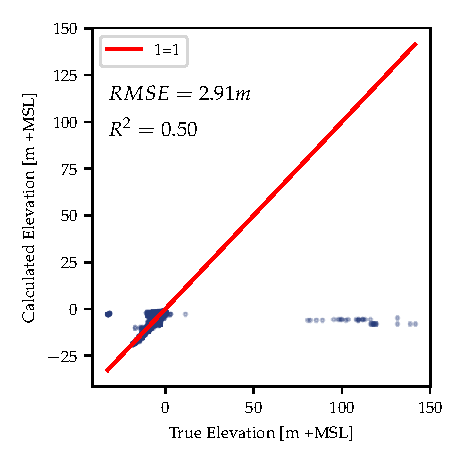
\includegraphics[width=0.45\textwidth]{figures/Oahu_combined_lidar_estimated_vs_truth.pdf}}{\caption{Bias plot of all points within all Oahu Subsites}\label{fig:oahu-bias-mountains}}
        \ffigbox{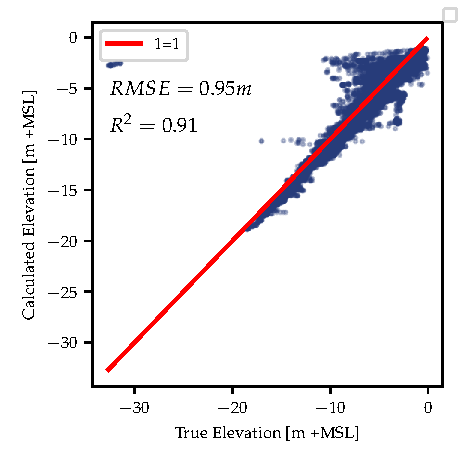
\includegraphics[width=0.45\textwidth]{figures/Oahu_combined_mountains_removed_lidar_estimated_vs_truth.pdf}}{\caption{Bias plot with the mountain points removed to better show the actual distribution of the error}\label{fig:oahu-bias-nomounts}}
    \end{floatrow}
\end{figure}

\section{Prediction of Lidar error}

One of the challenges of extracting bathymetry from ICESat-2 data is finding robust, automated ways of distinguishing between signal and noise. For the KDE approach utilized, a minimum kernel density threshold of $\max({kde_{50},0.10})$ was found to provide a good balance between filtering out the most severe errors and retaining as much data as possible. Increasing the minimum parameter to 0.15 was found to decrease RMS error of the ICESat-2 point bathymetry, but at the expense of throwing out significant amount of high quality data at the same time. Therefore, increasing the threshold was found to lower the error for the point data while simultaneously \emph{increasing} the error in the resulting kriging surface.

Therefore, better methods are required to predict the quality of the bathymetry data in coastlines without in-situ data. Two ways of approaching this are explored: analyzing which parameters predict the error at the level of an individual photon, and analyzing if certain variables predict the aggregate error of each transect. Improved filtering by transect would allow better discrimination of signal/noise, improving the quality of the output, while finding variables that indicate if a transect contains any bathymetry data would allow pre-filtering of the best transects, allowing the KDE signal finding approach to be scale to larger sites more efficiently.

\subsection{Per-photon error}
Several variables that are provided on a per-photon basis which might have some impact on the error at each photon. Two variables that were checked for their relationship to the error of a single photon are the count of photons in the 20 m segment (\emph{count\_ph} in the ATL03 data). This is the count of photons that are in the 20 m segment around the reference photon. An indication of the total count of photons could be useful to predict the presence of bathymetric signal, since fewer photons present in a segment might indicate data issues (e.g., interference from clouds) in the surrounding area.

To evaluate the effect, every single bathymetry point from all sites was combined. The comparison between the absolute error and the count of photons in the local 20 m segment is shown in Figure \ref{fig:error-photon}. The photons from Oahu subsite 2 with an error in the range 80--150 m have been removed from the data before plotting. Because the reason for the anomalously high error in these points is known, they will not examined any further here (For the reason for these errors see section \ref{sec:oahuresults}).

Looking at the other photons, clustered near the bottom of Figure \ref{fig:error-photon}, there is indeed a relationship between the photon count variable and the absolute error; the photons with higher absolute error (from 20--40 m) are all clustered near the left side of the graph, indicating that many of the photons with a large error occur in transects with a photon count from 0--200 photons. However, there is a large density of photons with a relatively low error value that are also in this range. Therefore, it presents the same tradeoff as increasing the kernel density threshold - increasing it will increase the quality of the data, but also requires throwing out a very significant amount of good data at the same time.

\begin{figure}[!ht]
    \centering
    \includegraphics{figures/error_full_sat_ph_count.pdf}
    \caption[Photon error vs segment photon count and the fraction of fully-saturated returns in the segment]{Left: Relationship between Photon count within 20 m segment and absolute error \\ Right: The number of full saturated photons in a segment vs the error at that point}
    \label{fig:error-photon}
\end{figure}

Another variable that was checked at the photon level is the percent of pulses within the segment that are determined to be fully saturated. This can also be an indication of data issues in the segment. However this variable is also not a good predictor of error in an individual photon, as seen in the left side of Figure \ref{fig:error-photon}. Part of the reason for this is that nearly all of the segments included here have a full saturation fraction of 0.0 (99.1\% of photons in all study sites).

\subsection{Per-transect error}

Another useful metric is understanding which transect-level variables could indicate high-quality bathymetry data within a transect. If some transect metadata variables are a strong indication of the quality of the bathymetric signal in the transect, this would allow filtering of transects before running the KDE algorithm, allowing a significant reduction of required computational resources. To calculate the transect-level statistics, all the signal photons are aggregated by the unique combination of date, site, and beam id. The unique combination of these three identifies a single transect at each site. The aggregate statistics are calculated to find the RMS error, the median Secchi disk depth, the average count of fully saturated photons, the photon density per meter, and the percent of high-confidence ocean photons. 

One variable that was checked at the transect level is the Secchi disk depth. The median Secchi disk depth was calculated for each unique transect, and then compared to the aggregate RMSE for that transect. The upper left side of Figure \ref{fig:track-level-stats} shows the resulting plot. For this purpose, the large magnitude errors from Oahu subsite 2 were removed, since they are caused by a known issue that is not related to the optical depth. The RMS error shows an even distribution across the entire range of Secchi depth values at the transect. Therefore there is no clear relationship between the median Secchi disk depth of a trackline and the RMS error of the ICESat-2 bathymetry data contained in that trackline, so this variable would not be useful to determine if a transect is likely to contain bathymetric signal.

\begin{figure}[!ht]
    \centering
    \includegraphics{figures/track-level-stats.pdf}
    \caption[Relationship between transect-level statistics and RMS error of ICESat-2 data]{Relationship between transect-level statistics and RMS error of ICESat-2 data. None of the investigated variables can serve as a good way to predict the presence or quality of bathymetric signal.}
    \label{fig:track-level-stats}
\end{figure}

The results of the photon-level analysis indicates the fraction of fully-saturated photons in the 20 m segment around a photon does not provide a good way to classify an individual photon as signal or noise. However, if many segments within a certain transect have a large fraction of saturated pulses, this indicates possible instrument errors along this transect. The average of the fraction of fully-saturated pulses for each unique transect was calculated. The upper right subfigure of Figure \ref{fig:track-level-stats} shows the relationship between this mean fraction of fully-saturated pulses and the RMS error in the transect. No significant relationship is found.

It was also hypothesized that the number of photons per meter of along-transect distance could provide a way to filter for high-quality data in a transect. It is inexpensive to calculate and indicates transects which consistently contain a high number of photons across their length with no significant horizontal gaps, which also likely indicates ideal data capture conditions since large horizontal gaps in signal are often induced by poor atmospheric conditions such as clouds or fog \parencite{atl03knownissues}. The density of photons per meter length for each transect was calculated. Its relationship with the transect RMS error is shown in the lower right of Figure \ref{fig:track-level-stats}. The plot shows that transects with a relatively high density relative to their length tend to have a lower RMS error. However, it does not serve as an effective way to filter: the majority of transects fall within the 0--5 m range, including those with very low RMSE and relatively high RMSE. Therefore using this value as a threshold would require filtering out many good transects to remove a handful of low-quality transects. 

Another variable which might provide a an indication of the presence of bathymetry signal in a given transect is the percentage of high-confidence ocean signal photons. This metadata variable is provided in  \emph{qa\_perc\_signal\_conf\_ph\_high} within the \emph{/quality\_assesment/} group in the ATL03 data. Generally, the ATL03 classification does not classify bathymetry signal points \emph{themselves} as high confidence ocean-surface photons (often, bathymetric signal points are classified as noise). However, there could be an indirect relationship between the percentage of high confidence ocean photons and the bathymetric signal quality because the percentage of high confidence ocean photons could be a proxy for the transect data quality in general (i.e., good atmospheric/weather conditions, no instrument issues, etc). The lower right side of Figure \ref{fig:track-level-stats} shows the relationship between the percentage of high confidence ocean signal photons and the RMS error. On the right side of the graph, it can be seen there are a large number of transects with a more than 95\% high confidence signal but still showing significant RMS error. Therefore, this variable does not provide a good way to determine which transects contain quality signal; any filtering based on the percent of high confidence ocean signal photons would remove significant amounts of high-quality transects, while leaving many of the lower quality transects.

Previous research on ICESat-2 bathymetry has found that the beam strength can affect the quality of the bathymetry data obtained. To investigate this relationship, the transects were grouped by this binary variable to find the RMSE of all strong beams and all weak beams. For this approach, it was found that the strong beams did have a slightly higher RMS error, but also were able to extract many more photons. Table \ref{tab:error-by-strongweak} shows the error metrics, and the total count of points found for each type of transect.

\begin{table}[!htb]
\centering
\caption{Error metrics per-transect based on beam type}
\label{tab:error-by-strongweak}
\begin{tabular}{lrrrr}
\toprule
Beam type & RMSE [m] & MAE [m] & ME [m] & Count of signal points \\
\midrule
Strong & 0.81 & 0.34 & 0.19 & 360,556 \\
Weak & 0.66 & 0.38 & 0.09 & 56,484 \\
\bottomrule
\end{tabular}
\end{table}



